\documentclass[11pt, professionalfonts]{beamer}
\usetheme[progressbar=head]{metropolis}
\useoutertheme{infolines}
\usecolortheme{beaver}

\usepackage{longtable}
% \usepackage{newtxtext,newtxmath}
\usepackage[backend=biber,
style=gb7714-2015, 
gbnamefmt=lowercase, 
maxcitenames=2,
mincitenames=1, 
gbcitelocal=gb7714-2015,
gbpub=false,
doi=false,
isbn=false,
url=false,
eprint=false]{biblatex}
\addbibresource{yy.bib}
\hypersetup{pdfpagemode=FullScreen}

\usepackage[fontset = none]{ctex}
\setsansfont{Source Han Serif SC}
\setCJKmainfont[ BoldFont = Source Han Serif SC Heavy, ItalicFont = FangSong]{Source Han Serif SC}
\usepackage[ruled, boxed]{algorithm2e}
\usepackage{graphicx}
\usepackage{amsmath}
\usepackage{amsfonts}
\usepackage{subfigure}
\usepackage{url}
\definecolor{awesome}{rgb}{1.0, 0.13, 0.32}
% \usepackage{mathptm}
\numberwithin{equation}{section}
\usefonttheme[onlymath]{serif}
% \setlength{\parskip}{1.2em}
\DeclareGraphicsExtensions{.eps,.ps,.jpg,.bmp,.png}

\author{统计71~王泽昊(指导教师: 张春霞)}
% \institute{指导教师: 张春霞}

\date{2021年6月22日}

\title{数学与统计学院~毕业设计答辩}
\subtitle[本科毕业设计]{聚类算法在地震速度谱自动拾取中的应用研究}

\graphicspath{{images/}}


\begin{document}
{\usebackgroundtemplate{\includegraphics[height=\paperheight,width=\paperwidth]{background.png}}
\maketitle

\begin{frame}[c]
    \frametitle{主要工作}
    \begin{itemize}
        \item 相关背景知识学习; 
        \vspace{10pt}\item 文献阅读, 文献翻译; 
        \vspace{10pt}\item 聚类算法理论学习; 
        \vspace{10pt}\item 代码编写, 进行试验; 
        \vspace{10pt}\item 探究可能改进方向. 
    \end{itemize}
\end{frame}

\section{问题背景介绍}

\begin{frame}[c]
    \frametitle{CMP道集}
    \begin{minipage}{.55\paperwidth}
        \begin{figure}[h]
            \centering
            \includegraphics[width = .9\textwidth]{03_共中点道集.png}
            \caption{Common MidPoint Gather}
        \end{figure}
    \end{minipage}
    \begin{minipage}{.35\paperwidth}
        Shot代表激发器, Receiver代表接收器, 每一对Shot-Receiver都呈对称分布. 
    \end{minipage}
\end{frame}

\begin{frame}[c]
    \frametitle{对应的速度谱}
    \begin{minipage}{.55\paperwidth}
        \begin{figure}[h]
            \centering
            \includegraphics[width = .9\textwidth]{04_偏移距与旅行时图像_NMO前.png}
        \end{figure}
    \end{minipage}
    \begin{minipage}{.35\paperwidth}
        Offset为偏移距, 即Shot-Receiver间的水平距离; Travel Time为旅行时, 即Shot发出的信号被Receiver接收到所需的时间. 
    \end{minipage}
\end{frame}

\begin{frame}[c]
    \frametitle{期望得到的速度谱}
    \begin{minipage}{.55\paperwidth}
        \begin{figure}[h]
            \centering
            \includegraphics[width = .9\textwidth]{05_偏移距与旅行时图像_NMO后.png}
        \end{figure}
    \end{minipage}
    \begin{minipage}{.35\paperwidth}
        将所有Shot-Receiver对得到的地震波记录都校正到同一旅行时上, 方便对所有地震波记录进行叠加. 
    \end{minipage}
\end{frame}

\begin{frame}[shrink]
    \frametitle{动校正}
    偏移距: $x$, 旅行时: $t$, 传播长度: $l$, 反射点深度: $h$, 零偏移距旅行时: $t_0$, 波速: $v$, 可以计算得到\cite{Green1938}: 

    \vspace{10pt}
    \begin{minipage}{.45\paperwidth}
        \begin{figure}[h]
            \centering
            \includegraphics[width = .9\textwidth]{06_旅行时计算公式.png}
        \end{figure}
    \end{minipage}
    \begin{minipage}{.45\paperwidth}
        \small
        \begin{equation*}
            t=\frac{l}{v}=\frac{2\sqrt{h^2+x^2/4}}{v}, t_0=2h/v, 
        \end{equation*}
        \begin{align*}
            t=\frac{2\sqrt{t_0^2v^2/4+x^2/4}}{v}=\sqrt{t_0^2+\frac{x^2}{v^2}}, 
        \end{align*}
        \begin{equation}
            t_0^2=t^2-\frac{x^2}{v^2}. 
            \label{equ:零偏距旅行时计算公式}
        \end{equation}
\end{minipage}
\end{frame}

\renewcommand{\algorithmcfname}{算法}
\begin{frame}[c]
    \frametitle{实际动校正过程}
    \begin{algorithm}[H]
        \KwIn{CMP道集, 动校正速度}
        \KwOut{动校正后的道集}
        \caption{实际动校正步骤}
        从动校正后的道集出发; \\
        \For{动校正后道集上的每一个点$(x,t_0)$}{
            用式~(\ref{equ:零偏距旅行时计算公式})~计算$t_0$在CMP道集上对应的旅行时$t$; 

            在CMP道集上找出点$(x,t)$关于$t$的前后两个点; 若个数不足则不进行后续步骤; 

            用前后两个点共四个点的振幅插值得到点$(x,t)$的振幅; 
            
            $(x,t)$的振幅就是校正后道集上点$(x,t_0)$的振幅。
        }
    \end{algorithm}
\end{frame}

\section{文献阅读、翻译}

\begin{frame}[c]
    \frametitle{文献调研}
    \vspace{10pt}
    通过阅读相关的外文文献, 了解到速度分析通常有以下几种方法: 
    
    \vspace{15pt}
    \begin{center}
        \begin{minipage}{.35\textwidth}
            \begin{itemize}
                \item 速度谱相似性; 

                \vspace{8pt}\item 局部地震斜率; 
                
                \vspace{8pt}\item 神经网络; 
                
                \vspace{8pt}\item 聚类. 
            \end{itemize}
        \end{minipage}
    \end{center}
\end{frame}

\begin{frame}[c]
    \frametitle{文献翻译}
    对下列两篇文献进行了全文翻译: 

    \vspace{20pt}
    \fullcite{Rodriguez2014}

    \vspace{20pt}
    \fullcite{Zhang2016}
\end{frame}

\section{背景、理论知识学习}

\begin{frame}
    \frametitle{背景知识学习}
    由于地震勘探学背景知识的缺乏, 对此书籍的前四章进行了学习: 

    \vspace{15pt}
    \fullcite{Zhou2014}
\end{frame}

\begin{frame}
    \frametitle{聚类算法理论学习}

    对于EM算法, 变分推断, Dirichlet过程的相关文献进行了阅读, 并对于相关的公式和算法进行了推导. 

    \vspace{10pt}
    \fullcite{Blei2006}

    \vspace{10pt}
    \fullcite{Blei2017}
\end{frame}


\begin{frame}{代码编写}
    代码编写目前约950行, 实现了对地震数据进行读取、预处理、聚类、结果分析、曲线拟合、在原始道集上进行NMO校正的功能. 曲线拟合和NMO校正的代码目前还不完善. 

    \vspace{15pt}\url{https://github.com/Addasecond86/XJTU-Bachelor-Dissertation-Statistics-WangZehao/tree/main/codes}
\end{frame}

\begin{frame}
    \frametitle{试验结果}
    % \begin{figure}[ht]
    %     \centering
    %     \subfigure[经过处理过后的最终聚类结果]{
    %         \includegraphics[height=6cm]{15_GMM_Dirichlet_TruePair_Centers_Real_n=35_n=9_CovType=diag_PriorType=dirichlet_process_Prior=0.03.pdf}
    %     }\ 
    %     \subfigure[曲线拟合结果]{
    %         \includegraphics[height=6cm]{16_GMM_Dirichlet_FittingMethod=Square_Curve_TruePair_Centers_Real_n=35_n=10_CovType=diag_PriorType=dirichlet_process_Prior=0.03_NoCombine.pdf}
    %     }
    % \end{figure}
\end{frame}

\begin{frame}
    \frametitle{试验结果}
    % \begin{figure}[ht]
    %     \centering
    %     \subfigure[原始道集]{
    %         \includegraphics[height=6cm]{17_Show.pdf}
    %     }\ 
    %     \subfigure[动校正后结果]{
    %         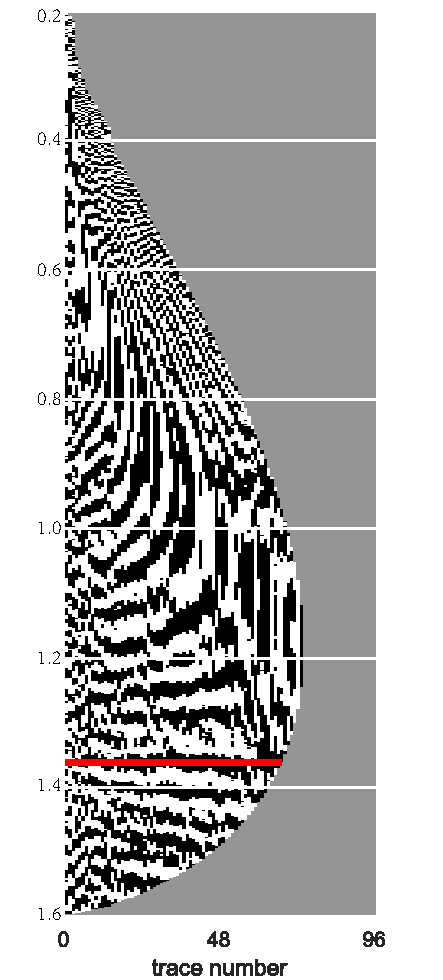
\includegraphics[height=6cm]{17_NMO.pdf}
    %     }
    % \end{figure}
\end{frame}

\begin{frame}[shrink]
    \frametitle{后续改进}

    \vspace{20pt}
    后续改进主要考虑在以下几个方面: 
    
    \vspace{20pt}
    \begin{center}
        \begin{minipage}{.6\textwidth}
            \begin{enumerate}
                \vspace{10pt}\item 完善曲线拟合与NMO校正的代码
                \vspace{10pt}\item 探究更加有效剔除噪声的方法
                \vspace{10pt}\item 探究更为合理的曲线拟合方法
            \end{enumerate}
        \end{minipage}
    \end{center}
\end{frame}

\printbibliography

\begin{frame}[plain,standout]
    \LARGE \emph{谢谢观看}
\end{frame}

\end{document}
